\chapter{Protezione Microdati}
\label{microdata_protection}

\section{Introduzione}

\section{Macrodata vs Microdata}

\section{Classificazione delle tecniche di protezione riguardo il Disclosure dei microdati}
Il controllo del disclosure dei microdati è un’importante problema pratico sia nel privato che nel pubblico.
$\\$
La protezione dei microdati ha apparentemente due obiettivi tra di loro contrastanti. Da una parte si vuole evitare la re-identificazione, la quale accade ogni qualvolta l’informazione del respondent che appare nella table di microdati è identificata; il quale, è associata con le identità dei respondent corrispondenti.
$\\$
Dall’altra invece le applicazioni di tecniche dovrebbero preservare le *chiavi delle proprietà statistiche* dei dati originali i quali sono state segnati come importanti dai destinatari dei dati (ossia chi riceverà i dati finali)

$\\$
Precisamente data una table di microdati T, una tecnica di protezione dei dati dovrebbe trasformare questa table T in una table $T_1$ in modo che:
\begin{enumerate}
    \item il rischio che un utente malevolo possa usare $T_1$ per determinare informazioni confidenziali o identificare un respondent, sia basso
    \item l’analisi statistica su T e $T_1$ possa produrre risultati simili
\end{enumerate}

Generalmente i seguenti fattori contribuiscono al rischio di disclosure:

\begin{itemize}
    \item L’esistenza di tuple altamente visibili (ossia tutte quelle tuple con caratteristiche che hanno caratteristiche uniche)
    \item Possibilità di matching tra le table di microdati e le informazioni esterne.
    \item L’esistenza di un alto numero degli attributi comuni che possono aumentare la possibilità di linking.
\end{itemize}

Mentre i fattori che minimizzano il rischio di disclosure sono:
\begin{itemize}
    \item Una table di microdati contenenti un subset della popolazione intera.
    Questo implica che le informazioni di un respondent specifico, il quale potrebbe essere un utente malevolo potrebbe voler sapere, potrebbe non essere incluso nella table di microdati.
    \item Le informazioni specificate nelle table rilasciate, quindi pubbiche non sono aggiormate. Potrebbero cambiare nel tempo, indi per cui il linking con le informazioni esterne potrebbero non essere accurati
    \item Una table di microdati e le informazioni esterne contengono rumore, riducendo la probabilità di linking delle informazioni
    \item Una table di microdati e le risorse esterne possono contenere dati espressi in forme diverse, riducendo l’abilità di linking
\end{itemize}

\begin{figure}[h]
    \centering
    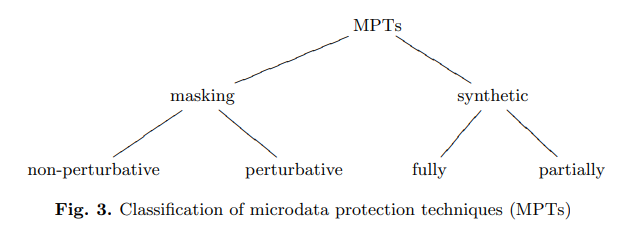
\includegraphics[width=0.5\linewidth]{paper_microdata/Fig3.png}
    \caption{Classificazione delle tecniche di protezione dei microdati}
    \label{fig:Fig 3}
\end{figure}

$\\$
Generalmente, per limitare il rischio di disclosure di una table di microdati è necessario sopprimere gli identifiers impliciti ed espliciti come step iniziale (e.g. SSN, Name)

$\\$
Questo processo  è noto come de-identificazione, quest’ultima non necessariamente rende le tuple anonime, siccome è possibile fare re-identificazione usando informazioni esterne.

$\\$
Tipicamente le tecniche sono basate sul principio che la re-identificazione possa essere contrastata riducendo la quantità delle informazioni rilasciate, mascherando i dati (e.g., non rilasciando o perturbando i valori), o rilasciando valori plausibili modificati invece di quelli reali. Seguendo questo principio le tecniche si suddividono in duo macro categorie: 
\begin{itemize}
    \item Tecniche di mascheramento: I dati originali sono trasformati producendo nuovi dati che non sono validi per le analisi statistiche in modo da preservare la confidenzialità dei respondent. Le tecniche di mascheramento si suddividono in:
    \begin{itemize}
        \item non perturbative: il dato originale non viene modificato, ma alcuni dati vengono soppressi o vengono rimossi dettagli.
        \item perturbativi: i dati originali sono modificati.
    \end{itemize}
    \item Generazione dei dati sintetici: I set di tuple originale nelle table di microdati sono sostituiti da un nuovo set di tuple generati in modo di preservare le proprietà statistiche chiave del dato originale.% Il processo di generazione è basato sui modelli statistici e le proprietà statistiche delle chiavi che non sono incluse nei modelli%
    Dal momento che le table dei microdati rilasciati contengono dati sintetici, il rischio di re-identificazione viene ridotto.
    Questi possono essere interamente sintetici (fully synthetic) o misti con i dati originali (partially synthetic).

    $\\$
    Un'altra caratteristica importante delle tecniche di protezione è che possono essere usati su tipo di dati differenti. In particolare i tipi di dati possono essere categorizzati come 
    \begin{itemize}
        \item \textit{Continui}: Un attributi è detto continuo se le operazioni numeriche e aritmetiche sono definite sull'attributo. E.g. Data di nascita e temperatura sono attributi continui.
        \item \textit{Categorici}: Un attributo è definito categorico se le operazioni aritmetiche non hanno alcun senso se fatto sull'attributo. E.g. Razza, su cui non si possono fare operazioni aritmetiche
    \end{itemize}
\end{itemize}
$\\$
Di seguito, sono descritti le tecniche di protezione dei microdati principali, e se sono applicabili a dati continui, categorici o entrambi.
\begin{figure}[h]
    \centering
    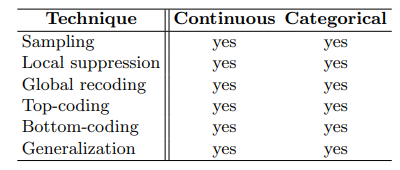
\includegraphics[width=0.5\linewidth]{paper_microdata/Fig4.png}
    \caption{Applicazione delle tecniche non perturbative su dati differenti}
    \label{fig:Fig-4}
\end{figure}

\begin{figure}[h]
    \centering
    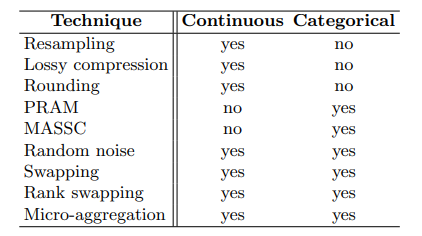
\includegraphics[width=0.5\linewidth]{paper_microdata/Fig5.png}
    \caption{Applicazione delle tecniche perturbative su dati differenti}
    \label{fig:Fig-5}
\end{figure}

\section{Tecniche di Mascheramento}
Alcune tecniche di mascheramento

\subsection{Tecniche non perturbative}
Le tecniche non perturbative producono microdati eliminando dettagli dai dati originali. Di seguito alcune di esse:

\begin{itemize}
    \item \textit{Sampling}: I table dei microdati protetti includono solo tuple formate da sample (campioni) della popolazione totale. Siccome c'è dell'incertezza se uno specifico respondent sia presente nei sample, il rischio di re-identificazione viene riudotto. Per esempio possiamo decidere se pubblicare solo le tuple pari della table originale. Questa tecnica può operare solo su dati categorici 
    
    \item \textit{Local suppression}: Sopprime i valori degli attributi in modo da limitare la possibilità di analisi. Questa tecnica lascia uno spazio vuoto su alcuni attributi (sensitive cells) che contribuiscono in modo significante al rischio di disclosure delle tuple coinvolte.
    
    \item \textit{Global Recoding}: Il dominio degli attributi, ossia tutti i possibili valori, sono divisi intervalli disgiunti di grandezza uguale, e ogni intervallo viene associato a una label. La table dei microdati protetti sono ottenuti sostituendo i valori degli attributi con le label associate agli intervalli corrispondenti. Questa tecnica riduce i dettagli della table e quindi riduce il rischio di re-identificazione. Sono presenti due tecniche particolari di recoding, ossia \textit{Top-Coding} e \textit{Bottom-Coding}, qui sotto descritte:
    \begin{itemize}
        \item \textit{Top-Coding}: E' basata sulla definizione di limite superiore (upper limit), chiamato top-code, per ogni attributo che deve essere protetto. Ogni valore maggiore di questo valore è sostituito dal top-code. Questa tecniche può essere applicata agli attributi categorici che possono essere ordinati linearmente come gli attributi continui.  
        \item \textit{Bottom-Coding}: Simile al top-coding ma definisce il limite inferiore (lower limit). Quindi, ogni valore più basso di questo non verrà ripubblicato e verrà sostituito con il bottom-code.
    \end{itemize}
    \item \textit{Generalization}: Consiste nel rappresentare i vaori di un dato attributo usando valori più generali. Questa tecnica è basata sulla definizione di generalizzazione gerarchica, dove i valori più generali sono alla radice della gerarchia e le foglie corrispondono ai valori specifici. Un processo di generalizzazione perciò procede con la sostituzione dei valori rappresentati dai nodi foglia con dei valori al nodo superiore.

    \begin{figure}[h]
        \centering
        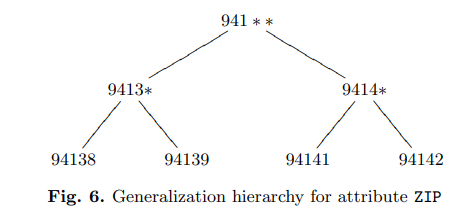
\includegraphics[width=0.5\linewidth]{paper_microdata/Fig6.png}
        \caption{Generalizzazione gerarchica}
        \label{fig:Fig-6}
    \end{figure}
\end{itemize}

\subsection{Tecniche perturbative}
Con le tecniche perturbative le table dei microdati vengono modificate per la pubblicazione
Le modifiche possono portare a combinazioni dei valori originali uniche le quali svaniscono non appena vengono introdotte nuove combinazioni.
\begin{itemize}
    \item \textit{Resampling}: Questa tecnica sostituisce i valori degli attributi sensibili continui con un valore medio computato sul numero di samples della popolazione originaria. Precisamente, assumiamo che $N$ sia il numero di tuple presenti in una table di microdati, e $S_1,...,S_t$ con $t$ i sample di dimensione $N$. Ogni sample viene rankato indipendentemente e successivamente viene calcolata la media del $j_{esimo}$ valore ranked. I valori medi ottenuti sono riordinati prendendo in considerazione l'ordine dei valori originali, seguendo quindi l'ordinamento della tabella iniziale.
    \begin{figure}[h]
        \centering
        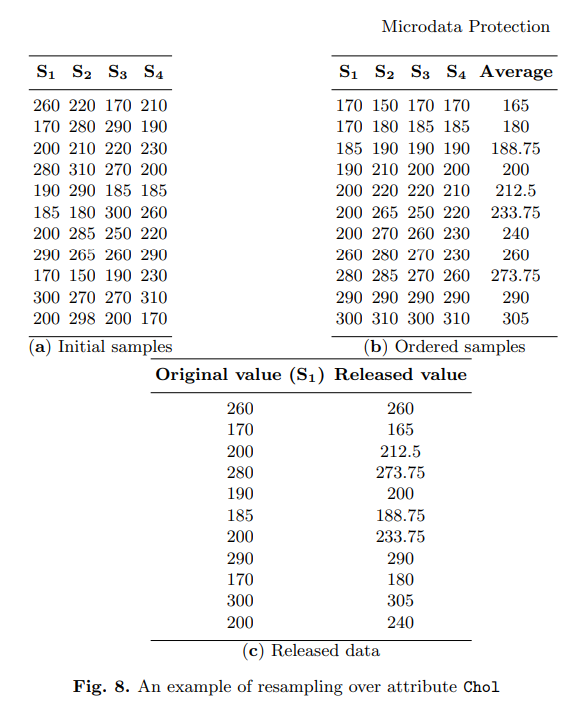
\includegraphics[width=0.5\linewidth]{paper_microdata/Fig8.png}
        \caption{Esempio di resampling}
        \label{fig:Fig-8}
    \end{figure}
    \item \textit{Rounding}: Simile alla tecnica usata anche per la protezione dei macrodati ed è applicabile solo agli attributi continui. Sostituisce i valori originali con dei valori approssimati, quest'ultimi sono scegli da un set di \textit{rounding points} $p_i$ ognuno il quale definisce il \textit{rounding set}. Per esempio: 
    \begin{itemize}
        \item \textit{\textbf{Rounding Points}} possono essere scelti come multipli di un valore base $b$, con $b = p_{i+1} - p_i$.
        \item \textit{\textbf{Rounding Sets}} definiti come 
        $\\$
        \begin{itemize}
            \item 
            $\begin{cases}
                [p_i - \frac{b}{2}, p_i + \frac{b}{2}) \text{con } i = 2,...,r-1 \\
                [0, p_1 + \frac{b}{2}) \\
                [p_r - \frac{b}{2}, X_{max}], \text{con } X_{max} \text{  il valore più grande possibile}
            \end{cases}$
            \item rispettivamente per $p_1$ e $p_r$
            \item Un valore $v$ di $X$ viene sostituito dal round point corrispondente al rounding set dove è contenuto $v$.
        \end{itemize}
    \end{itemize}
    
    \item \textit{Random Noise}: Perturba gli attributi sensibili aggiungendo o moltiplicando una variabile casuale con una distribuzione. Il rumore additivo (additive noise) è preferito al rumore moltiplicativo (multiplicative noise) e viene formalmente definito così:
    $\\$
   \textit{Poniamo $X_j$ come la $j_{esima}$ colonna della table dei microdati originaria corrispondente a un attributo sensibile e supponiamo che ci siano $N$ tuple.
    Ogni valore $X_{ij}$, con $i$ = $1,...,N$, viene sostituito con $x_{ij}$ + $\varepsilon_{ij}$, dove $\varepsilon_j$ è il vettore degli errori normalmente distribuiti ricavati da una variabile casuale con la media uguale a 0, in generale, con una varianza che sia proporzionale agli attributi originari}
    
    $\\$

    \textit{Forse da approfondire}
    
    \footnote{N.B $\epsilon$ viene usato per perturbare i dati ma lasciando intatta la correlazione con la tabella iniziale}
    
    \item \textit{Swapping}: Consiste nel modificare il subset di una table di microdati facendo lo swapping dei valori di un set formato degli attributi sensibili, chiamato \textit{swapped attributes}, tra coppie di tuple selezionate (le coppie sono selezionate secondo un criterio ben definito).
    Intuitivamente, questa tecnica riduce il rischio di re-identificazione perché introduce dell'incertezza sul valore reale legato al dato del respondent. Anche se questa tecnica è facile da applicare, generalmente ha lo svantaggio di non preservare le proprietà dei sottodomini. Inizialmente la tecnica originale fu presentata solamente per gli attributi categorici.
    
    \item \textit{Micro-Aggregation (o Blurring)}: Consiste nel raggupprare le tuple individiduali in piccole aggregazioni di una dimensione fissata $k$: verrà pubblicata la media di ogni aggregato invece dei valori individiduali. Anche se esistono diverse funzioni per caloclare la similrità, può essere difficile trovare un soluzione di raggruppamento ottimale. 
    Ci sono diverse varianti di \textit{micro-aggregation}, per esempio la media può sostituire il valore originale anche solo per una singola tupla nel gruppo o per tutte.
    Molti attributi possono essere protetti grazie a \textit{micro-aggregation} usando lo stesso o un diverso raggruppamento e, la dimensione del gruppo puo essere variabile o fissata ad un minimo. 
\end{itemize}
    
\section{Tecniche per la Generazione di Dati Sintetici}
La generazione dei dati sintetici è una valida alternaitiva per la protezione dei microdati. Il principio base su cui queste tecniche sono basate riguarda la non correlazione tra i contenuti statistici dei dati e l'informazione provvista da ogni respondent, quindi un modello ben rappresentante il dato potrebbe sostiture il dato stesso. Un requisito molto importante per la generazione dei dati sintetici, che rende il processo di generazione un problema importante, è che i dati sintetici e il dato originale potrebbero presentare la stessa qualità delle analisi statistiche. Il vantaggio maggiore di questi tipi di tecniche è che i dati sintetici rilasciati non sono collegati a nessun respondent, indi per cui il rilascio non può essere soggetto al fenomeno di re-identificazione; questo, inoltre, lascia ai proprietari dei dati di porre maggiore attenzione sulla qualità del dato rilasciato, invece che al problema di re-identificazione.

\section{Misure per valutare la confidenzialità e l'utilità dei Microdati}
Come discusso precedentemente, ci sono svariate tecniche per la protezione dei microdati. Le performance di queste tecniche di protezione sono valutate in termini di \textit{information loss} e \textit{disclosure risk}.
\begin{itemize}
    \item Information loss è la quantità di informazioni che esistono nei microdati originali e che, a causa delle tecniche di protezione, questo non si verifica nei microdati protetti.
    \item Disclosure risk è il rischio di incorrere nel disclosure quando i micordati vengono rilasciati.
\end{itemize}

Esistono due soluzioni estreme per il rilascio di microdati, le quali sono: 
\begin{itemize}
    \item Crittare i dati originali (rimuove il rischio di disclosure e il massimo di information loss)
    \item Rilasciare i dati originali (massimo rischio di disclosure e nessun information loss)
\end{itemize}
$\\$
In questa sezione andremo a descrivere alcuni dei pmetodi più importanti usati per quantificare il rischio di disclosure e di perdita di informazione (information loss).

\subsection{Rischio di Disclosure (Disclosure Risk)}
Generalmente ci sono due tipi di disclosure: \textit{disclosure di identità} e\textit{disclosure di attributi}. Il disclosure riguardo l'identita si occupa di una specifica identità la quale può essere linkata a tuple presenti nelle table di microdati. La disclosure riguardo gli attributi invece l'informazione che può essere spifferata di un attributo legato ad un individuo. In generale, due fattori che potrebbero avere un impatto sul disclosure di identità sono: 
\begin{itemize}
    \item \textit{univocità della popolazione}, ossia la probabilità di identificare un respondent, il quale è unico, con una specifica combinazione di attributi è elevata se quei attributi sono presenti nella table di microdati.
    \item \textit{re-identificazione}, ossia, che i mcirodati rilasciati sono linkabili ad un'altra table pubblicata, dove gli \textit{identifiers} non sono stati rimossi.
\end{itemize}
$\\$
Sono stati proposti diversi metodi per misurare il rischio di disclosure dei microdati rilasciati. Per esempio, \textit{la combinazione minima non sicura degli attributi} ritorna il numero degli attibuti con una combinazione unica presenti in una specifica tupla di microdati.
Questo metodo può essere adottato solo con le tecniche di mascheramento non perturbative, e, più è alto questo valore tanto più basso sarà il rischio di disclosure.

$\\$
\textit{\textbf{Univocità}}
$\\$
Ogni qual volta un sample unico è anche una popolazione unica, il disclosure d'identità diventa molto più probabile. Esistono metodi differenti per valutare il rischio di univocità, e tutti i metodi si affidano alla valutazione della probabilità.
\noindent Il primo metodo misura la probabilità dell'univocità della popolazione (\textit{population uniqueness (PU)}), ossia la probabilità che nella popolazione esista solo un individuo con una certa combinazione di valori su un determinato insieme di attributi. Questa probabilità è misurata come:
\\ $Pr(PU)$ = $\sum_{j}I$, con $\frac{F_j = 1}{N}$, dove $N$ è la dimensione della popolazione e $F_j$ è il numero degli individui nella popolazione con la $j_{esima}$ combinazione sugli attributi considerati, e $I()$ è una funzione e:
\\
$\begin{cases}
    I(A) = 1, \text{ se } A = true \\
    0, \text{ altrimenti.}
\end{cases}$
\\
\\Il secondo metodo misura la probabilità che un sample unico \textit{sample unique (SU)} sia anche una popolazione unica \textit{(PU)}. questa probabilità è misurata come: \\
$PR(PU|SU) = \frac{\sum_{j}I(f_j = 1, F_j = 1)}{\sum_{j}I(f_j = 1)}$,
dove $f_j$ è il numero degli individui presenti nei sample con la $j_{esima}$ combinazione sugli attributi considerati.
\\
\\Questi metodi sono chiamati misure \textit{file-level} perché assegnano lo stesso rischio a tutte le tuple. Il rischio di disclosure \textit{tuple-level} è la probabilità di disclosure dell'identità di un individuo specifico.\\
Questi tipi di misure sono state introdotte a causa della non-omogeneità del rischio di re-identificazione su un'intera tabella di microdati.\\ 
Supponendo che ci siano $K$ combinazioni differenti dei valori legati ai quasi-identifiers. Queste combinazioni producono una suddivisione sia nella popolazione che nei sample. Assumendo che $F_k$ sia la frequenza della $k_{esima}$ suddivisione, il rischio di disclosure per una tupla presente in un sample con la $k_{esima}$ combinazione è $\frac{1}{F_k}$.
\\ Il problema di questo metodo è che $F_k$ non è generalmente noto per la popolazione. Poiché le frequenze della distribuzione campionaria $f_k$
sono note, si considera la distribuzione delle frequenze $F_k$, data $f_k$ ($F_k|f_k$ può essere modellata come una binomiale negativa).
\\
\\Si noti che l'univocità può essere utilizzata come misura del rischio di divulgazione solo solo se i microdati sono stati protetti attraverso una 
tecnica di mascheramento non perturbativa.\\
Le tecniche perturbative modificano i valori dei dati e quindi non è possibile stabilire correttamente la frequenza di un valore nel campione rilasciato, perché possono essere introdotte nuove combinazioni uniche e possono scomparire le combinazioni uniche originali.
\\
\\\textit{\textbf{Record Linkage}}
\\
Consiste nel trovare un match tra le tuple presenti nelle table di microdati protetti e le tuple presenti nelle fonti esterne di informazione pubbliche e non anonime. Poiché non è possibile conoscere a priori tutte le fonti esterne di informazione che possono essere utilizzate da un eventuale utente malintenzionato, viene eseguito un controllo probabilistico sui microdati protetti.\\
È necessario adottare diversi metodi di record linkage a seconda che la tabella di microdati e le informazioni esterne abbiano o meno attributi comuni. Se ci sono attributi comuni, è necessario innanzitutto adottare una rappresentazione unica per gli attributi comuni. Ad esempio, abbreviazioni diverse nel nome di una persona porterebbero a concludere che due tuple non sono correlate, mentre in realtà si riferiscono allo stesso respondent. È quindi possibile adottare una strategia per il record linkage. I metodi di record linkage possono essere suddivisi in tre grandi categorie:
\begin{itemize}
    \item \textit{deterministici}: Cerca una corrispondenza esatta su uno o più attributi tra tuple di diversi set di dati. Il principale svantaggio di questo metodo è che non prende in considerazione la rilevanza dell'attributo nel trovare un collegamento.
    
    \item \textit{probabilistici}: Dati due dataset, $D_1$ e $D_2$, viene calcolato l'insieme di tutte le possibili coppie di tuple ($d_{1i}$, $d_{2j}$ ), dove
    \\
    $\begin{cases}
        d_{1i}$ $\in$ $D_1 \\
        d_{2j}$ $\in$ $D_2. 
    \end{cases}$ 
    \\
    \\A ogni coppia è associata una probabilità che rappresenta se la coppia è una corrispondenza reale. 
    \begin{itemize}
        \item Se la probabilità è inferiore a una soglia fissa $T_1$, la coppia viene scartata perché le tuple sono considerate non linked
        \item Se la probabilità è superiore a una seconda soglia fissa $T_2$, la coppia è considerata una corrispondenza reale
        \item Se la probabilità è compresa tra $T_1$ e $T_2$, è necessaria una valutazione umana per verificare se rappresenta una corrispondenza o meno. Tale probabilità viene calcolata considerando diversi pesi per i vari attributi e l'accordo o l'accordo parziale sui valori degli attributi. I pesi associati agli attributi e le due soglie $T_1$ e $T_2$ sono stabiliti dal proprietario dei dati.
    \end{itemize}
    
    \item \textit{basati sulla distanza}: Dati due insiemi di dati, $D_1$ e $D_2$, ogni tupla $d_{1i} \in D_1$ viene abbinata alla tupla più vicina $d_{2j} \in D_2$.\\ 
    Questo metodo richiede la definizione di una funzione di distanza $f$ tra coppie di tuple. Per esempio, la definizione di $f$ può sfruttare funzioni di distanza definite sugli attributi e può assegnare pesi diversi a ciascun attributo, a seconda della sua importanza nel processo di link. Un esempio di funzione di distanza è la \textit{Distanza Euclidea}, che considera ogni tupla come un vettore e assegna lo stesso peso a ogni attributo. Questo metodo di record linkage non è adatto agli attributi categorici, perché è difficile definire la distanza tra due categorie, in particolare se il loro dominio non è ordinato.
    \\Vengono usati anche altri metodi quando ci sono dataset senza attributi comuni. In questi casi la re-identificazione è più difficile. Un metodo proposto di recente si basa sul clustering. Fondamentalmente, un metodo di clustering viene applicato ai set di dati considerati. Il risultato è un insieme di cluster di tuple e ogni cluster all'interno di un set di dati viene mappato su un cluster all'interno dell'altro set di dati. Tale mappatura viene eseguita utilizzando una funzione di similarità. Sebbene il record linkage sia considerato una minaccia, ci sono molte situazioni in cui può essere utile. Il record linkage può essere utilizzato nella gestione di grandi database per estrarre informazioni importanti sullo stesso soggetto. Ciò è particolarmente utile quando i dati sono distribuiti su server diversi (ad esempio, le informazioni mediche della popolazione sono solitamente distribuite su sistemi diversi e una tecnica di record linkage può essere sfruttata per ricostruire le informazioni associate a un determinato individuo).
\end{itemize}
$\\$
\textit{\textbf{Interval Disclosure}}
\\
La misura di disclosure dell'intervallo viene calcolata in modi diversi, a seconda del tipo di dato dell'attributo (contino o categorico).\\
Nel caso di attributo categorico, per ogni tupla presente nella table di microdati, gli intervalli classificati (\textit{ranked intervals}) sono costruiti come segue.\\
Ogni attributo è classificato indipendentemente e un intervallo classificato è definito attorno il valore assunto dall'attributo in ogni tupla $t$. I ranghi dei valori all'interno dell'intervallo costruito intorno alla tupla t devono differire meno del p\% del numero totale di tuple.\\
Inoltre, il rango al centro dell'intervallo deve corrispondere al valore assunto dall'attributo considerato nella tupla $t$. Il rischio di divulgazione è quindi la proporzione dei valori originali che cadono nell'intervallo centrato sul valore protetto corrispondente. Se tale proporzione è pari al 100\%, un potenziale aggressore(attacker) è sicuro che il valore originale si trovi nell'intervallo attorno al valore protetto.\\
Nel caso di dati continui, il metodo è simile al precedente. La differenza principale è il modo in cui vengono costruiti gli intervalli classificati: non è possibile sfruttare il ranking e la costruzione si basa sulla deviazione standard dell'attributo.

\subsection{Perdita di Informazione (Information Loss)}
La misura per la perdita di informazione è strettamente correlata allo \textit{scopo} per cui l'informazione verra usata. Poiché gli scopi potrebbero essere differenti a non conosciuti a priori, non è possibile stabilire una misura generale per la perdita di informazione basata sul solo scopo. I metodi usati sono quindi, basati sui concetti di \textit{analiticamente validi} e \textit{analiticamente interessanti}, cui vengono definiti come seguono:
\begin{itemize}
    \item una tabella di microdati protetta è analiticamente valida se conserva approssimativamente le analisi statistiche (ad esempio, media e covarianza) che possono essere prodotte con i microdati originali;
    \item una tabella di microdati protetta è analiticamente interessante se contiene un numero suffience di attributi che possono essere validamente analizzati.
\end{itemize}

Generalmente, ci sono due strategie per calcolare la perdita di informazione:
\begin{enumerate}[label=\textit{\roman*)}]
    \item confrontando direttamente le tuple dei microdati protetti con le tuple dei microdati originali.
    \item confrontando le statistiche calcolate sui micordati protetti con le stesse statistiche valutate sui microdati originali.
\end{enumerate}
Descriviamo ora l'idea di base di alcune delle più comuni misure di perdita di informazioni, suddivise in due categorie in base al tipo di dati degli attributi. Sono stati proposti altri metodi, sia per tecniche specifiche di protezione dei microdati sia per casi generici.
\\
\\\textit{\textbf{Dati Continui}}
\\
Per misurare la perdita di informazioni, la statistica di interesse (ad esempio, matrici di co-varianza, matrici di correlazione o loro varianti) viene valutata sia sui dati originali che su quelli protetti e la differenza tra i due valori viene calcolata. Le discrepanze tra le due statistiche possono essere valutate in tre modi diversi: 
\begin{itemize}
    \item \textit{errore quadratico medio}
    \item \textit{errore medio assoluto}
    \item \textit{variazione della media}
\end{itemize}
Oltre alle misure statistiche, i dati possono essere confrontati prima e dopo l'applicazione di una tecnica di protezione dei microdati, calcolando nuovamente la differenza con uno dei tre metodi sopraccitati.
È importante notare che il valore della perdita di informazioni deve avere un valore massimo (ad esempio, 100 se si utilizza una notazione percentuale) per confrontare metodi diversi che hanno la stessa scala di calcolo della perdita di informazioni.
\\
\\\textit{Dati Categorici}
\\
Le misure di perdita di informazione introdotte brevemente per gli attributi continui non sono direttamente applicabili agli attributi categorici. In questo caso, le misure principali sono tre: 
\begin{itemize}
    \item \textit{confronto diretto}
    \item \textit{confronto tra tabelle di contigenza}
    \item \textit{misura di entropia}
\end{itemize}
Il confronto diretto dei valori degli attributi categoriali richiede la definizione di una funzione di distanza tra le categorie. Nel caso di categorie non ordinate, la distanza tra la categoria $c_1$ nei microdati originali e la corrispondente categoria $c_2$ nei microdati protetti è:
\\
$\begin{cases}
    \text{uguale a } 0, \text{ se le due categorie sono le stesse}\\
    1, \text{ altrimenti}
\end{cases}$
\\
\\Al contrario, se esiste un ordinamento tra le categorie, la distanza tra le categorie $c_1$ e $c_2$ è pari al numero di categorie tra $c_1$ e $c_2$ diviso per il numero totale di categorie. La misura di confronto delle tabelle di contingenza consiste nel confrontare le tabelle di contingenza corrispondenti. Una misura basata sull'entropia può essere utilizzata quando una tabella di microdati è stata protetta applicando le tecniche di soppressione locale, global recoding o PRAM. L'idea è che la perdita di informazione possa essere misurata utilizzando l'\textit{entropia di Shannon}, poiché il processo di mascheramento viene modellato come il rumore aggiunto ai microdati originali quando vengono trasmessi attraverso un canale rumoroso. La misura della perdita di informazione utilizza la probabilità condizionale (la probabilità di un valore nei microdati originali, una volta che il valore nei microdati protetti è dato).

\subsection{Combnazione di Rischio di Disclosure e Perdita di Informazione}
Le tecniche di protezione dei microdati descritte in questo capitolo hanno un impatto diverso sull'utilità dei dati e sul rischio di divulgazione. Per poter valutare tecniche alternative di protezione dei microdati, abbiamo bisogno di un quadro di riferimento per valutare la bontà di una tecnica di protezione.\\ 
Il rischio di divulgazione e la perdita di informazioni devono quindi essere combinati. Un metodo semplice consiste nel calcolare la media dei due valori e scegliere la tecnica (e l'impostazione dei parametri) con il punteggio più alto. Un altro metodo è quello delle \textit{mappe di confidenzialità R-U}, che è un grafico in cui la misura dell'utilità dei dati (l'inverso della perdita di informazioni) è riportata sull'asse $x$ e il rischio di divulgazione è riportato sull'asse $y$. Per ogni tecnica di protezione dei microdati, viene tracciata una linea sul piano cartesiano con un punto per ogni parametro impostato. Sulla base del grafico ottenuto, è possibile confrontare le varie tecniche di protezione e scegliere la più adatta. Una volta scelta la tecnica di protezione, le mappe di riservatezza R-U possono essere utilizzate anche per la selezione dei parametri. È importante notare che una mappa R-U è solo un metodo per correlare il rischio di divulgazione e la perdita di informazioni; tali misure devono essere calcolate utilizzando uno dei metodi sopra menzionati.\\
Un altro approccio per bilanciare l'utilità dei dati e il rischio di divulgazione è rappresentato dal concetto di tabella $k$-minima con $k$-anonimity (guarda il capitolo “$k$-anonimity”). Il $k$-anonimity stabilisce una soglia limite inferiore di rischio di divulgazione per una tabella, assicurando che ogni tupla della tabella non possa essere correlata a meno di $k$ rispondenti. L'approccio alla k-anonimità mira a trovare (applicando tecniche di generalizzazione e soppressione) una tabella $k$-minima, cioè una tabella che non generalizza più di quanto sia necessario per raggiungere la soglia $k$. In altre parole, una tabella $k$-minima è una tabella che minimizza la perdita di informazioni.\\
\\
\\Le misure descritte dovrebbero essere utilizzate prima che i dati vengano rilasciati per verificare se la protezione è adeguata alle "richieste di riservatezza dei respondent e alle esigenze di informazione dei destinatari dei dati".\\
Dopo l'applicazione delle tecniche di protezione , i micordati protetti possono essere controllati e rilasciati solo se sono conformi ad un certo grado di protezione. Queste misure possono essere usate anche dal destinatario dei dati per valutare la "protezione dei respondent e l'utilità dei dati"

\section{Conclusioni}
Oggi le società globali interconnesse hanno una grande richiesta sulla disseminazione e la condivisione di informazioni. Mentre nel passato le informazioni rilasciate erano principalmente in forma tabulare e statistica, molte situazioni oggi chiamano per il rilascio dei microdati specifici. 
Per affrontare questo problema sono state proposte numerose tecniche di protezione e, in questo capitolo, sono state descritte le tecniche di base per la protezione contro il disclosure dei microdati, classificando queste in tecniche di mascheramento e tecniche di generazione di dati sintentici. Per riassumere, le tecniche di generazione di dati sintentici proteggono i dati trasformando i loro valori. D'altro canto le tecniche di generazione di dati sintentici proteggono i dati sostituendoli con nuovi dati i quali conservano le proprietà statistiche originali. Inoltre sono state illustrate anche le principali misure adottate, solitamente, per valutare la riservatezza dei dati e l'utilità dei microdati protetti.